\documentclass[11pt]{article}
\usepackage{setspace}
\usepackage{pxfonts}
\usepackage{graphicx}
\usepackage{geometry}

\geometry{letterpaper,left=.5in,right=.5in,top=1in,bottom=.75in,headsep=5pt,footskip=20pt}

\vspace{-1in}
\title{Problem Set 5 -- Extensions of the Hodgkin-Huxley model}
\author{Computational Neuroscience Summer Program}
\date{June, 2011}

\begin{document}
\maketitle

In this problem set you will be extending the standard Hodgkin-Huxley model you constructed in Problem Set 4.  In this extended model we will be simulating the actions of individual voltage-dependent Sodium and Potassium channels.  Feel free to re-use any code from Problem Set 4 that you think would be useful.  Write up your results in a text editor of your choosing.  Include any relevant figures.  Include a printout of your Matlab code as well as any calculations that aren't in the code.  You may work individually or in groups, but each student should hand in their own report.

\subsection*{Equations}

\begin{center}
\begin{tabular}{l|l|l}
$\tau_x(V)\frac{dx}{dt} = x_\infty(V) - x$ & $\tau_x(V) =
\frac{1}{\alpha_x(V) + \beta_x(V)}$ & $x_\infty(V) =
\frac{\alpha_x(V)}{\alpha_x(V) + \beta_x(V)}$ \\
\hline
$\alpha_n(V) = \frac{.01(V+55)}{1 - exp(-.1(V+55))}$ &
$\alpha_m(V) = \frac{0.1(V+40)}{1 - exp(-.1(V+40))}$ &
$\alpha_h(V) = 0.07*exp(-.05(V+65))$\\ 
\hline
$\beta_n(V) = 0.125*exp(-.0125(V+65))$ &
$\beta_m(V) = 4*exp(-.0556(V+65))$ &
$\beta_h(V) = \frac{1}{1 + exp(-.1(V+35))}$\\
\hline
$P_K = n^4$ & $P_{Na} = m^3h$ &\\
\hline
$g_K = \bar{g}_KP_K$ & $g_{Na} = \bar{g}_{Na}P_{Na}$ &\\

\end{tabular}
\end{center}

\subsection*{Problems}

\paragraph{1.} Construct and simulate the stochastic K$^+$ channel model as shown in the state diagram below.  The diagram shows transitions between different states of a K$^+$ channel.  The symbols $\alpha_n$ and $\beta_n$ represent the opening and closing rates, respectively, of individual K$^+$ channels (these are the same variables you used in Problem Set 4).  Set the rate constants equal to their value at 10 mV (i.e., use $\alpha_n(10 \mathrm{mV}) = 0.65$/ms and $\beta_n(10 \mathrm{mV}) = 0.05$/ms).  Transitions are made between states with each iteration of your program if a random number chosen uniformly between 0 and 1 is less than the corresponding rate for that transition time.  For example, if a channel is in state 1, that channel will transition to state 2 during the current iteration of your program if the chosen random number is less than $4\alpha_ndt$.  As the channel(s) make transitions between states, keep track of whether state 5 is occupied.  If so, assume that each channel conducts 1 pA (10$^{-12}$ A) of current; otherwise no current flows through the channel.  Plot currents generated by this model for $N = $1, 10, and 100 channels over a 20 ms period (use $dt = 0.01$ ms).

\begin{figure}[h]
\begin{center}
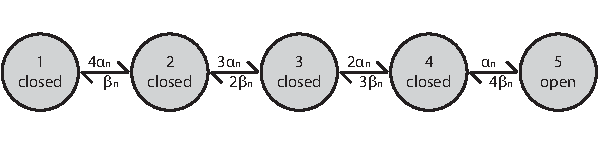
\includegraphics[width=0.5\textwidth]{hodgkin_huxley_advanced/K_state_diagram}
\end{center}
\end{figure}

\paragraph{2.}  The Hodgkin-Huxley description of the K$^+$ channel predicts the current flowing in these simulations would be $Nn^4$ pA, where $N$ is the number of  K$^+$ channels and $n$ is the K$^+$ activation variable (same as in Problem Set 4).  On a single plot, show the amount of current predicted by the Hodgkin-Huxley prediction and the amount of current predicted with the stochastic model.  (Use $N = 1000$.)

\paragraph{3.}  Construct an stochastic Na$^+$ channel model analogous
to the K$^+$ model, using the state diagram below.  The symbols $\alpha_m$ and $\beta_m$ represent
opening and closing rates of the three main subunits of the sodium
channel.  Activation and deinactivation rates of the sodium channel
gate are represented by $k_1$, $k_2$, and $k_3$.  Set the rate
constants equal to their value at 10 mV (i.e., use $\alpha_m(10
~\mathrm{mV}) = $5.034/ms, $\alpha_h(10~\mathrm{mV}) = $0.0016/ms, and $\beta_m(10~\mathrm{mV}) = $0.0618/ms).  Use
$k_1 = 0.24$/ms, $k_2 = 0.4$/ms, and $k_3 = 1.5$/ms.  As the channel(s) make transitions between states, keep track of whether state 4 is occupied.  If so, assume that each channel conducts -1 pA (10$^-{12}$ A) of current; otherwise no current flows through the channel.  Plot currents generated by this model for $M = $1, 10, and 100 channels over a 20 ms period.

\begin{figure}[h]
\begin{center}
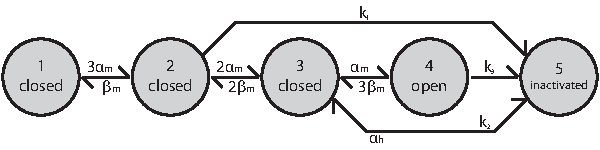
\includegraphics[width=0.5\textwidth]{hodgkin_huxley_advanced/Na_state_diagram}
\end{center}
\end{figure}

\paragraph{4.}  The Hodgkin-Huxley description of the Na$^+$ channel
predicts the current flowing in these simulations would be $-Mm^3h$ pA,
where $M$ is the number of Sodium channels.  On a single plot, show the amount of current predicted by the Hodgkin-Huxley prediction and the amount of current predicted with the stochastic model.  (Use $M = 1000$.)

\paragraph{5.  Challenge problem.}  Modify the Hodgkin-Huxley model from Problem Set 5 to explicitly simulate Sodium and Potassium channels using the stochastic models above (to start, use $N = M = 1000$).  You will need to update the transition probabilities $\alpha_n, \alpha_m, \alpha_h, \beta_n,$ and $\beta_m$ with each time step, since those transition probabilities are voltage-dependent.  $k_1, k_2,$ and $k_3$ are constants.  Hint: $P_X$ is equal to the total proportion of $X$ channels  currently open.  Simulate a 20 ms interval.  Apply an external current of $I_{ext} = 5$ nA/mm$^2$ from 5 to 8 ms.  Plot $V$, $P_K$, and $P_{Na}$ as a function of time.  

\end{document}


